\subsection{Outcome analysis} \label{subsection: Outcomes}

In this section we cover the analysis of the game outcomes (win, lose, tie), both under the fairness aspect and the performance of strategies.

\begin{figure}
	\centering
	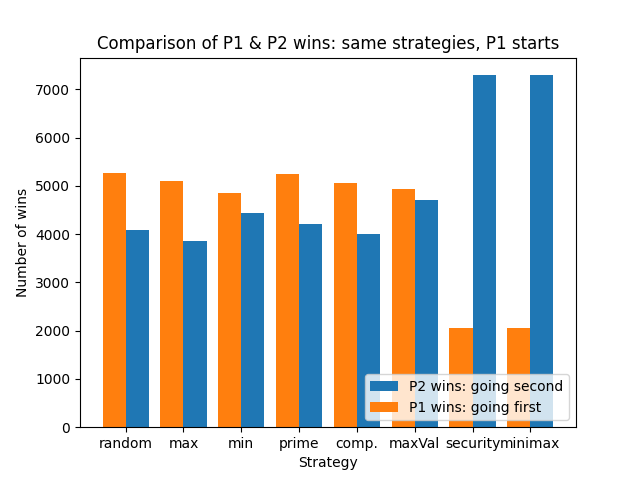
\includegraphics[width=1\linewidth]{img/histogram_p1vsp2_p1first.png}
	\caption{Number of wins of P2 vs P1 when P1 starts; both players play the same strategy.}
	\label{fig:hist_p1vsp2_p1first}
\end{figure}

\begin{figure}
	\centering
	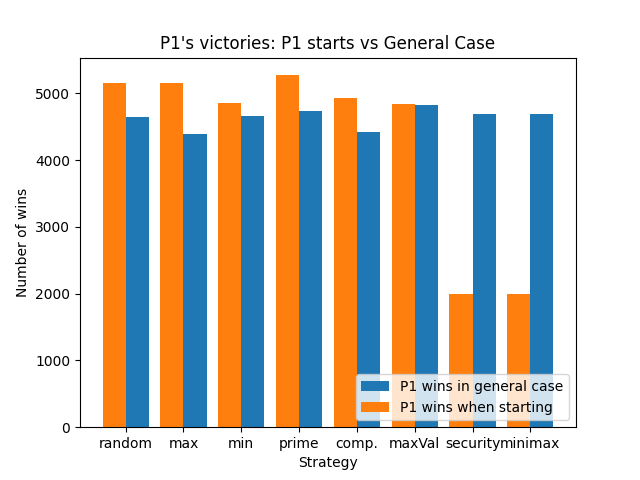
\includegraphics[width=1\linewidth]{img/histogram_p1wins_2cases.png}
	\caption{Number of wins of P1 when starting vs the general case; both players play the same strategy.}
	\label{fig:hist_p1wins_2cases}
\end{figure}

%\begin{figure}
%	\centering
%	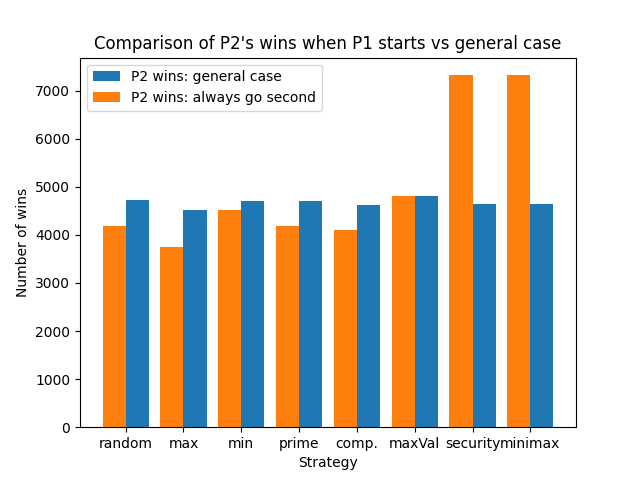
\includegraphics[width=1\linewidth]{img/histogram_p2wins_2cases.png}
%	\caption{Number of wins of P2 when P1 starts vs the general case; both players play the same strategy.}
%	\label{fig:hist_p2wins_2cases}
%\end{figure}

 Our analysis starts by considering Figures \ref{fig:hist_p1vsp2_p1first} and \ref{fig:hist_p1wins_2cases} where the two players play the same strategies.
 Those figures highlight the following points about the fairness of the game:
 \begin{itemize}
 	\item There is an advantage in going first for some strategies, i.e. random, max, min, prime, comp;
 	\item The situation is more or less balanced when playing the max\_value strategy;
 	\item There is a significant advantage in going second when both players play a either the security or minimax strategy;
 \end{itemize}
 A combined observation of the first and second point is quite interesting: it seems that there is an advantage in going first when using stupid primitive strategies, but for more advanced ones the situation is flipped. An accurate analysis of this behaviour is quite difficult, given in particular the random nature of some of the strategies, however we propose an intuition to motivate it: a player using more advanced strategies and going second takes more opportunities to strategically form arithmetical operations with the cards visible on the table, considering also the potential opponent response, and thus achieve a greater number of points right from the first turns. This intuition is also supported by the more or less balanced behaviour of the max\_val pair, where each player tries to get the maximum partial payoff out of the current game state but without strategically looking ahead on the consequences of its action.

\begin{figure}
	\centering
	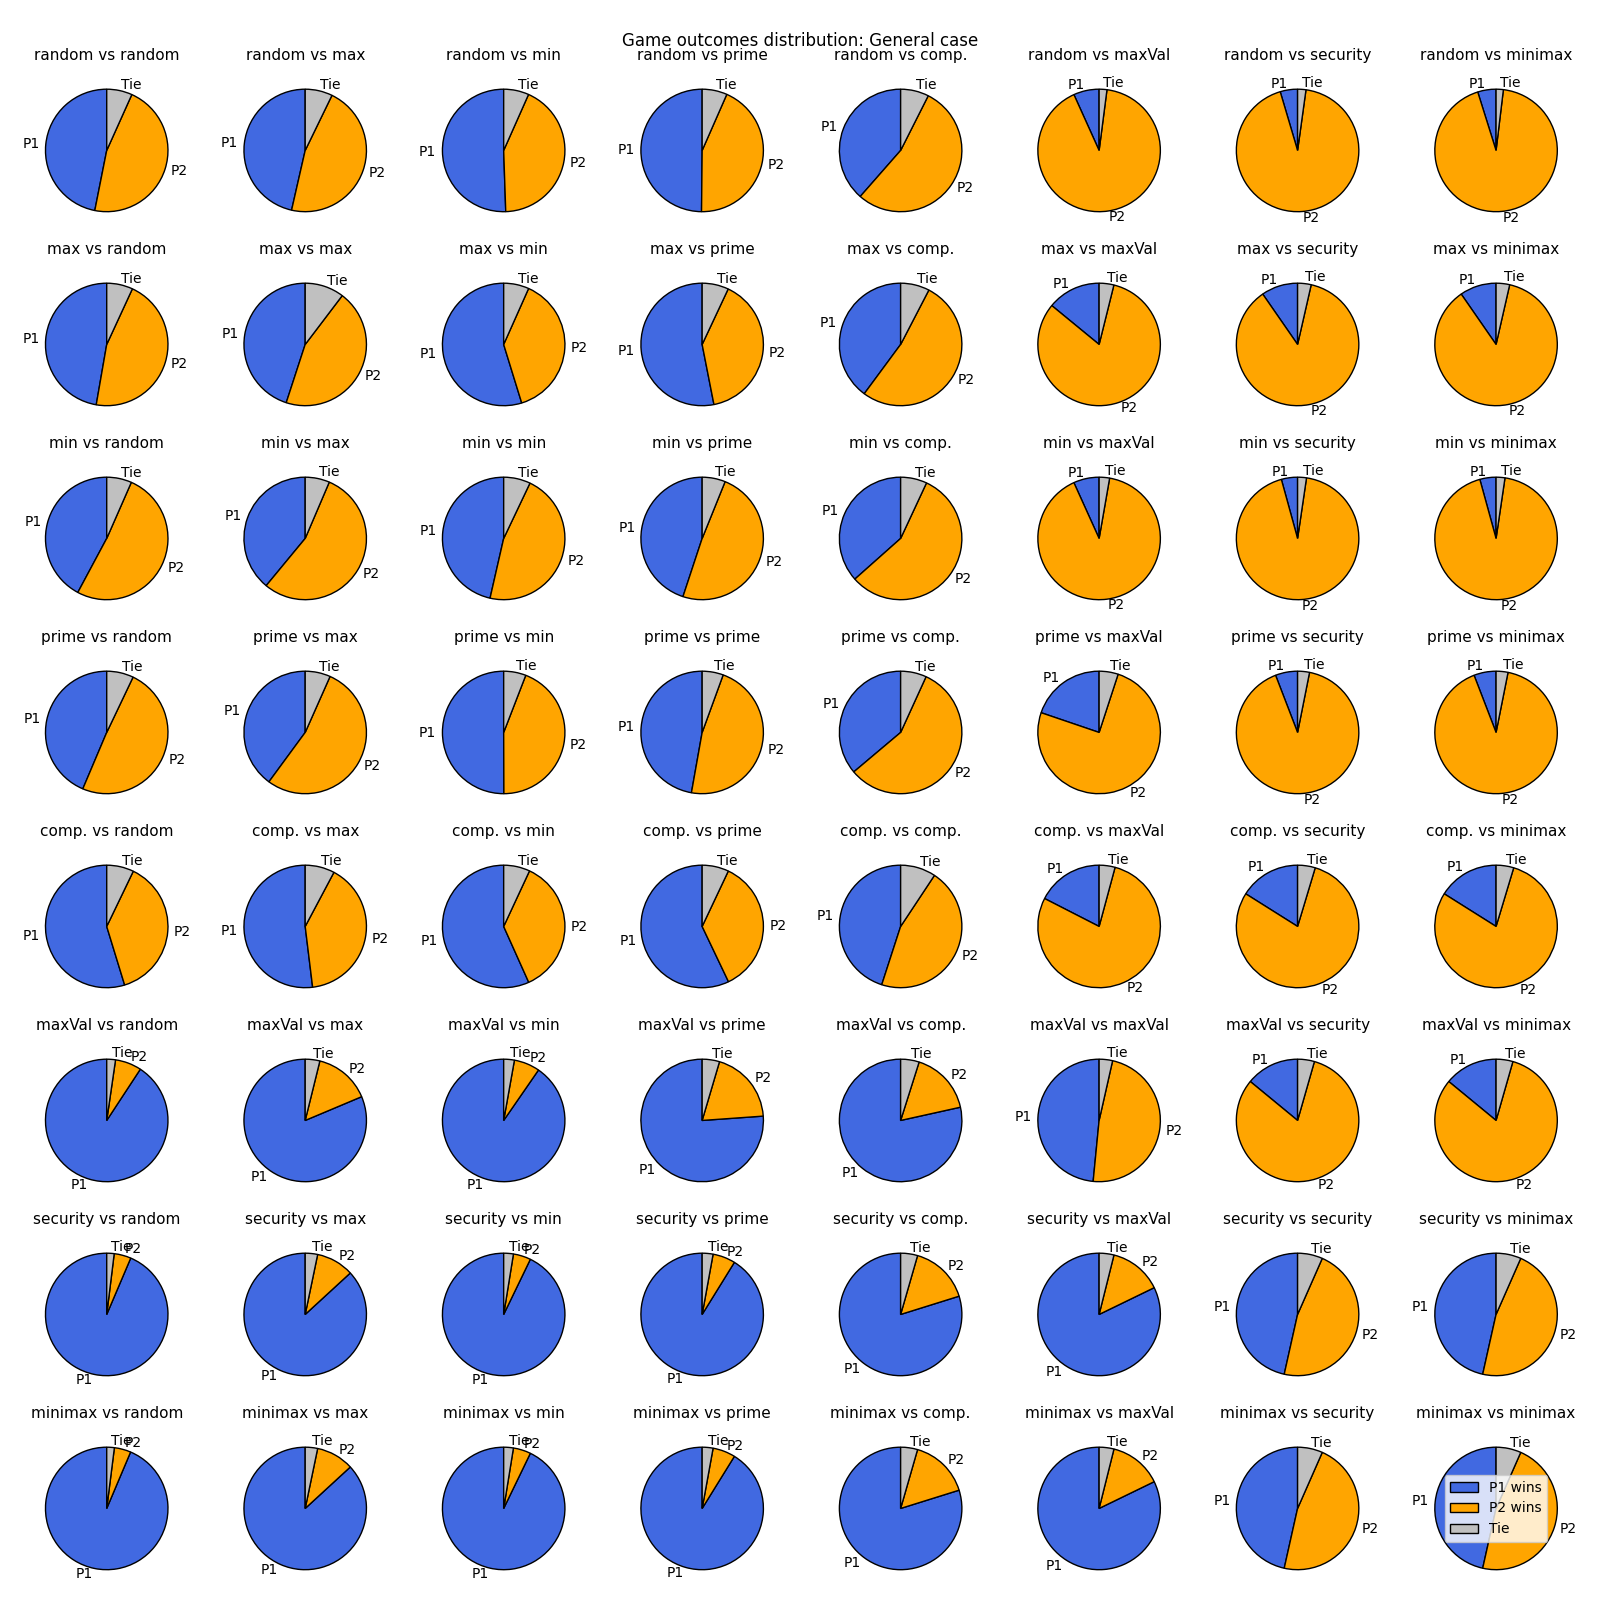
\includegraphics[width=1\linewidth]{img/outcomes_distribution_general.png}
	\caption{Outcomes distribution under all possible strategies combinations in the general case.}
	\label{fig:outcomes_distribution_general}
\end{figure}

\begin{figure}
	\centering
	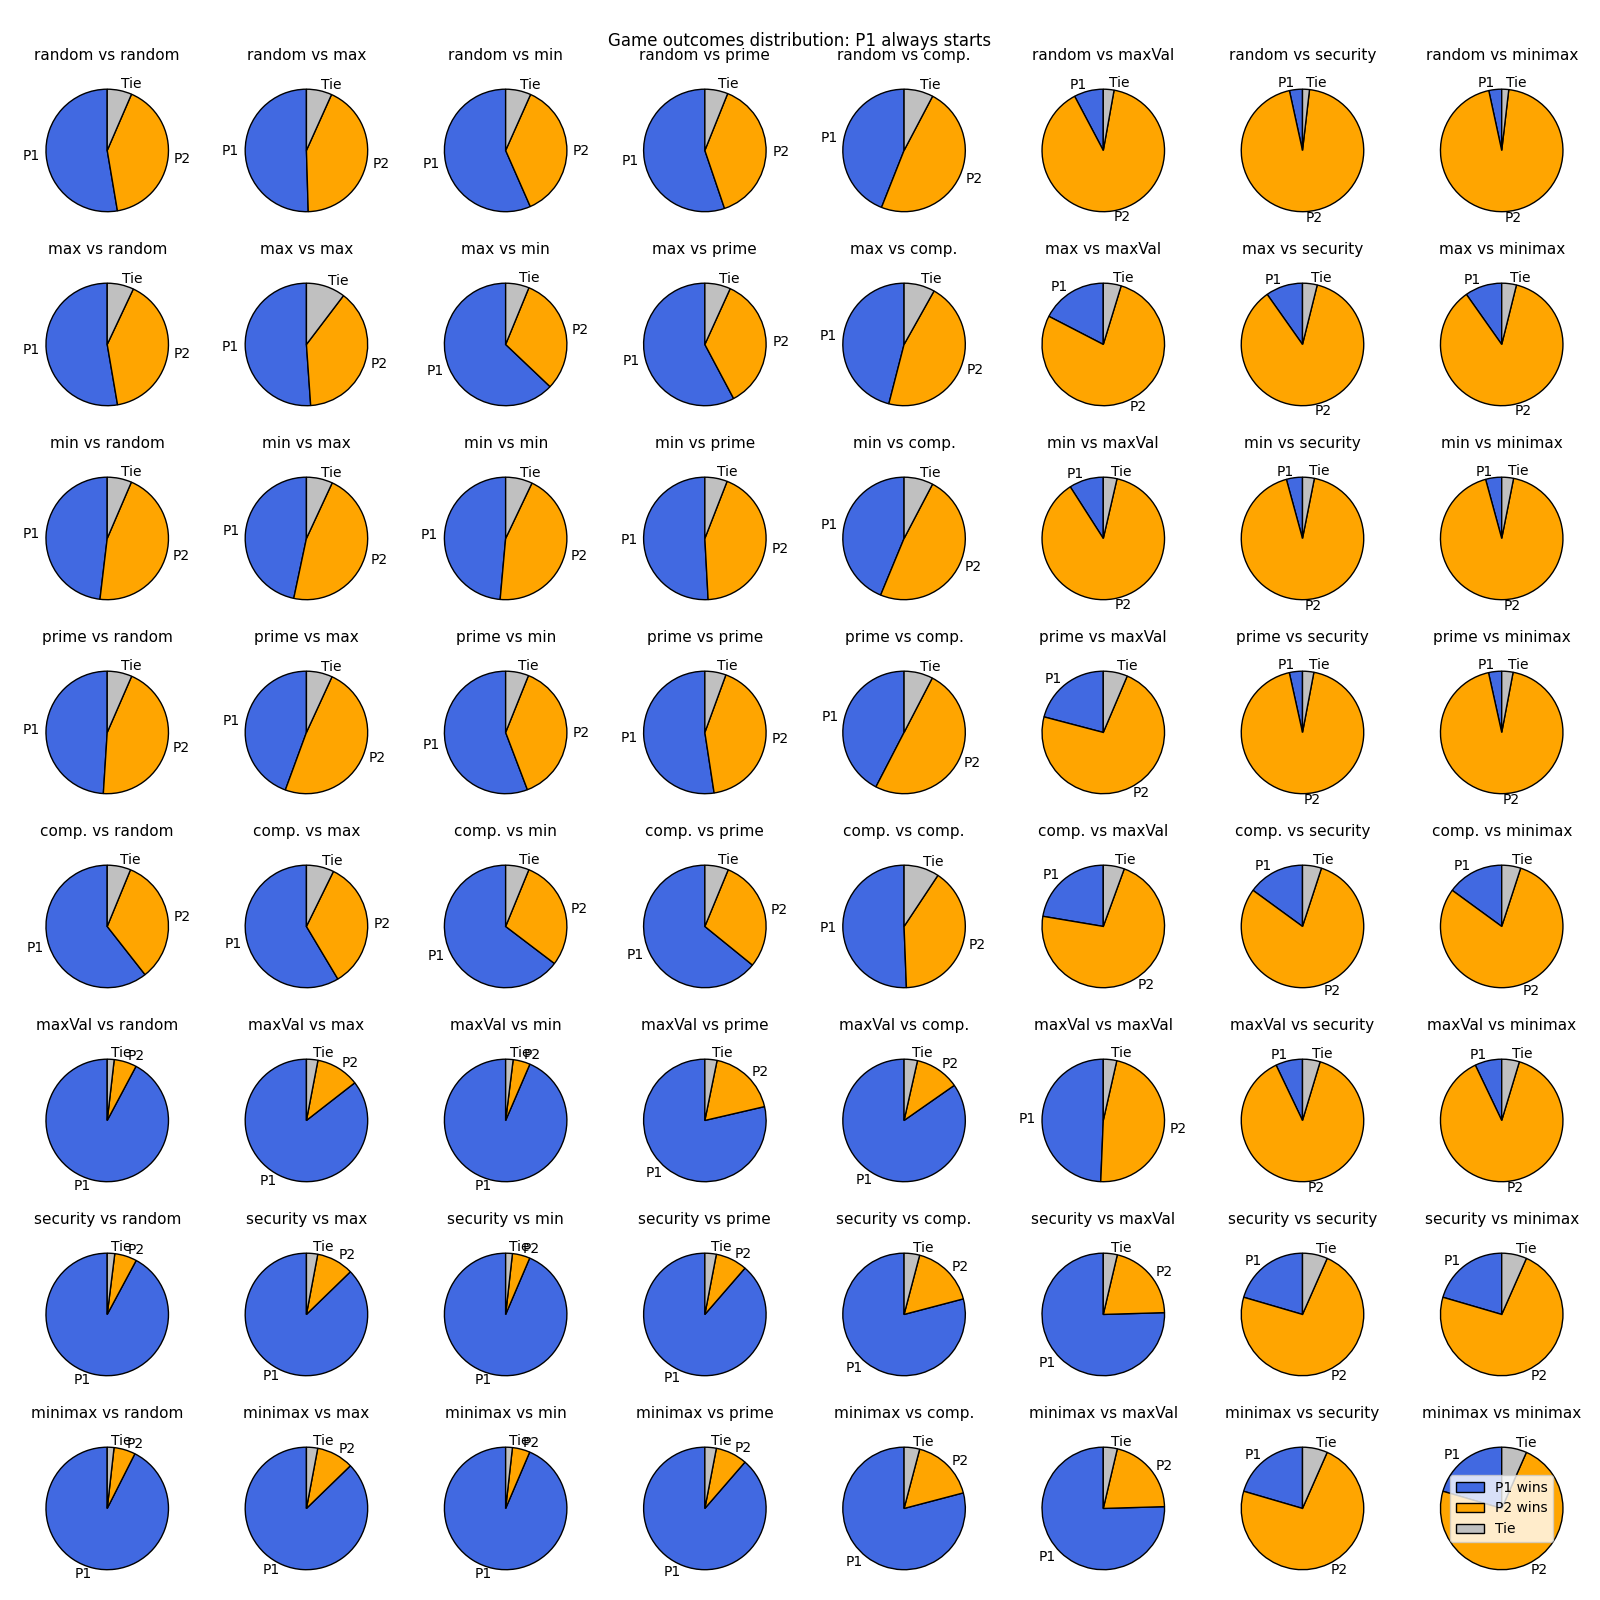
\includegraphics[width=1\linewidth]{img/outcomes_distribution_p1first.png}
	\caption{Outcomes distribution under all possible strategies combinations when P1 starts.}
	\label{fig:outcomes_distribution_p1first}
\end{figure}

Figures \ref{fig:outcomes_distribution_general} and \ref{fig:outcomes_distribution_p1first} strength those observations and expand on them, by allowing to see the distribution of wins for each player under all possible strategies combinations, in the general and P1-first cases respectively.
In particular, it is easy to see that there is an evident advantage in using zero-sum-like strategies in both cases. This was expected, since those two practical strategies are the ones that approximate more closely actual best-response strategies.
Additionally, we can see again the advantage in always going second when playing such strategies.

On the same note, also the max\_val	strategy performs quite well against the more primitive strategies, being based on the idea of "best play in a vacuum"; however, it gets outperformed by the zero-sum strategies, an expected result given their nature.

More importantly, those two figures allow us to discuss the fairness of the game on the whole: when considering the diagonals of the two figures (in other words players playing the same strategy), we clearly see that in the general case the situation is always more or less balanced, something that we do not see when we force P1 to go first. This allows us to conclude that the game is fair on the whole, but this fairness is more related to the randomized nature of whoever starts, i.e. whoever gets the 2 card, rather than the intrinsic characteristics of the game.

\begin{figure}
	\centering
	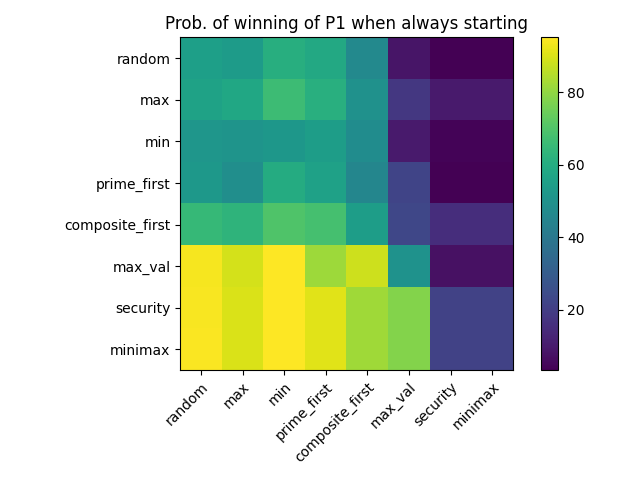
\includegraphics[width=1\linewidth]{img/prob_p1first.png}
	\caption{Heatmap of the probability of P1 winning when always going first.}
	\label{fig:prob_p1first}
\end{figure}

\begin{figure}
	\centering
	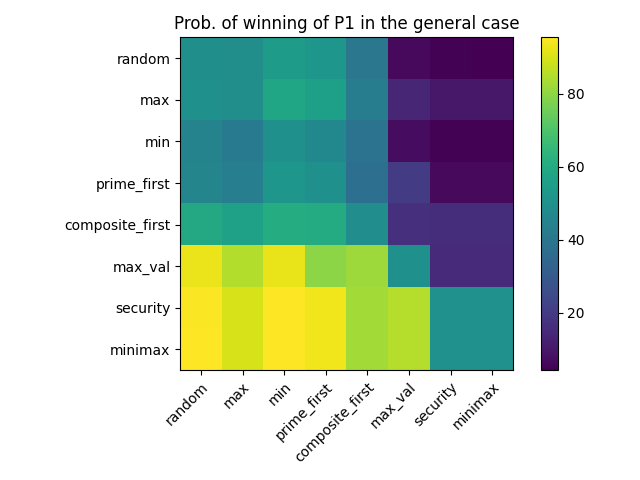
\includegraphics[width=1\linewidth]{img/prob_general.png}
	\caption{Heatmap of the probability of P1 winning in the general case.}
	\label{fig:prob_general}
\end{figure}

\begin{figure}
	\centering
	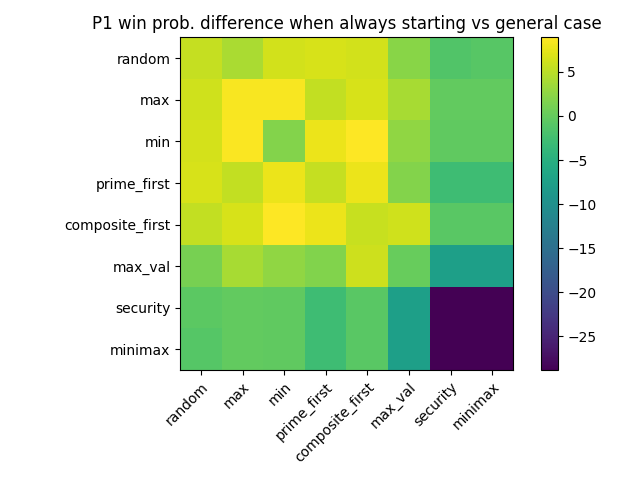
\includegraphics[width=1\linewidth]{img/prob_diff.png}
	\caption{Difference in probability of P1 winning when always going first vs in the general case.}
	\label{fig:prob_diff}
\end{figure}

In Figures \ref{fig:prob_general} and \ref{fig:prob_p1first} we show the probability of P1 winning under all the different strategy combinations as heat-maps for the two study cases.
The situation that we are presented with is quite similar to the one that we presented in Figures \ref{fig:outcomes_distribution_general} and \ref{fig:outcomes_distribution_p1first}, additionally highlighting the symmetrical situations across the diagonals.

However, the most interesting result is presented in Figure \ref{fig:prob_diff}, where the difference in victory probability of P1 between the P1-always-starts case and the general case is shown. The key takeaways are:
\begin{itemize}
	\item When considering simple primitive strategies, there is a slight advantage by always going first;
	\item When considering the more advanced strategies, there is a great difference in probability of victory between always starting and the general case, favouring going second;
\end{itemize}

To wrap up the outcomes analysis:
\begin{itemize}
	\item We have shown that more skilled players, i.e. players using advanced strategies, significantly outperform players using more simple strategies;
	\item Interestingly enough, we have seen that between low skilled players using primitive strategies the first one to move is favoured, however, the situation flips as soon as skilled players with advanced strategies come into play, favouring going second;
	\item Randomizing the hands, and thus whoever starts (general case), makes the game fair on the whole when considering players of "same skill level" (in other words, strategies of comparable complexity); however, this has more to do with the properties of randomization than the innate characteristics of the game.
\end{itemize}